\section{Direct products and direct sums}
\begin{ex}
    $S_{3}$ is not the direct product of any family of its proper subgroups. The same is true of $Z_{p^{n}}$($p$ prime, $n\geq 1$) and $\mathbb{Z}$.
\end{ex}

\begin{answer}
    We list all the subgroups of $S_{3}$: $\{(1), (12)\}$, $\{(1), (13)\}$, $\{(1), (23)\}$, $\{(1), (123), (132)\}$. Only $\{(1), (123), (132)\}$ is normal, so $S_{3}$ isn't an direct product of any family of its proper subgroups.

    For $Z_{p^{n}}$, $Z_{p^{i}}\lhd Z_{p^{n}}$ for all $i=1,2,\dots ,n-1$ but $Z_{p^{i}}\cap Z_{p^{j}}\neq \{e\}$. So $Z_{p^{n}}$ isn't an direct product of any family of its proper subgroups.

    For $\mathbf{Z}$. $\forall N_{1}\lhd \mathbf{Z}$, $N_{2}\lhd \mathbf{Z}$, we have $N_{1}=\left\langle a_{1}\right\rangle$ and $N_{2}=\left\langle a_{2}\right\rangle$. Thus, $N_{1}\cap N_{2}=\left\langle a_{1}a_{2}\right\rangle\neq \{e\}$. So $\mathbf{Z}$ isn't an direct product of any family of its proper subgroups.
\end{answer}

$$ $$

\begin{ex}
    Give an example of groups $H_{i}$, $K_{i}$ such that $H_{1}\times H_{2}\cong K_{1}\times K_{2}$ and no $H_{i}$ is isomorphic to any $K_{j}$.
\end{ex}

\begin{answer}
    Take $H_{1}\cong K_{1}\times K_{2}$, $H_{2}=\{e\}$. We verify that $H_{1}\times H_{2}\cong K_{1}\times K_{2}$. There exists $f:H_{1}\to K_{1}\times H_{2}$ which is an isomorphism. There exists canonical projection $\pi_{1}:H_{1}\times H_{2}\to H_{1}$ and $\pi_{1}$ is an epimorphism. $\mathrm{Ker}\pi_{1}=\{(e_{1},e_{2})\}$ thus $\pi_{1}$ is also a monomorphism. Therefore $\bar{f}=f\circ \pi_{1}$ is a well defined isomorphism. $H_{1}\times H_{2}\cong K_{1}\times K_{2}$ but neither $H_{1}$ nor $H_{2}$ are isomorphic to any $K_{i}$, $i=1,2$.
\end{answer}

$$ $$

\begin{ex}
    Let $G$ be and (additive) abelian group with subgroups $H$ and $K$. Show that $G\cong H\oplus K$ if and only if there are homomorphisms 
    
    \begin{figure}[H]\centering
        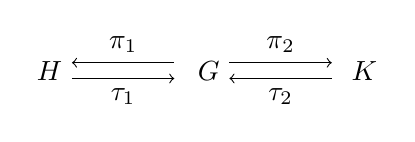
\begin{tikzpicture}
            \node [left] at (0,1) {$H$};
            \node [left] at (2,1) {$G$};
            \node [left] at (4,1) {$K$};
            \draw [<-] (0,1.1)-- node [above, pos=0.5]{$\pi_{1}$} (1.3,1.1);
            \draw [->] (0,0.9)-- node [below, pos=0.5]{$\tau_{1}$} (1.3,0.9);
            \draw [->] (2,1.1)-- node [above, pos=0.5]{$\pi_{2}$} (3.3,1.1);
            \draw [<-] (2,0.9)-- node [below, pos=0.5]{$\tau_{2}$} (3.3,0.9);
        \end{tikzpicture}
    \end{figure}
    such that $\pi_{1}\tau_{1}=1_{H}$, $\pi_{2}\tau_{2}=1_{K}$, $\pi_{1}\tau_{2}=0$ and $\pi_{2}\tau_{1}=0$, where 0 is the map sending every element onto the zero (identity) element, and $\tau_{1}\pi_{1}(x)+\tau_{2}\pi_{2}(x)=x$ for all $x\in G$.
\end{ex}

\begin{answer}
    If $G\cong H\oplus K$. Denote $f:G\to H\oplus K$ which is a isomorphism. Then there are canonical products $\pi_{1}'$, $\pi_{2}'$, $\tau_{1}'$, $\tau_{2}'$. 

    \begin{figure}[H]\centering
        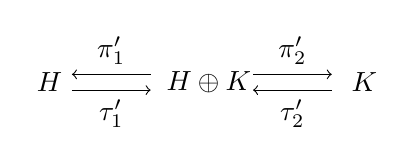
\begin{tikzpicture}
            \node [left] at (0,1) {$H$};
            \node [left] at (2.4,1) {$H\oplus K$};
            \node [left] at (4,1) {$K$};
            \draw [<-] (0,1.1)-- node [above, pos=0.5]{$\pi_{1}'$} (1,1.1);
            \draw [->] (0,0.9)-- node [below, pos=0.5]{$\tau_{1}'$} (1,0.9);
            \draw [->] (2.3,1.1)-- node [above, pos=0.5]{$\pi_{2}'$} (3.3,1.1);
            \draw [<-] (2.3,0.9)-- node [below, pos=0.5]{$\tau_{2}'$} (3.3,0.9);
        \end{tikzpicture}
    \end{figure}
    Thus

    \begin{figure}[H]\centering
        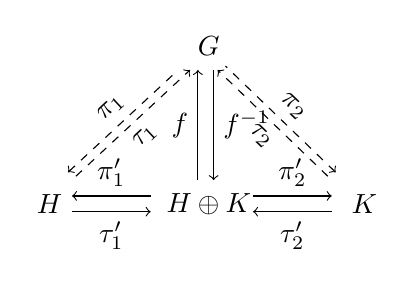
\begin{tikzpicture}
            \node [left] at (0,1) {$H$};
            \node [left] at (2.4,1) {$H\oplus K$};
            \node [left] at (4,1) {$K$};
            \node [left] at (2,3) {$G$};
            \draw [<-] (0,1.1)-- node [above, pos=0.5]{$\pi_{1}'$} (1,1.1);
            \draw [->] (0,0.9)-- node [below, pos=0.5]{$\tau_{1}'$} (1,0.9);
            \draw [->] (2.3,1.1)-- node [above, pos=0.5]{$\pi_{2}'$} (3.3,1.1);
            \draw [<-] (2.3,0.9)-- node [below, pos=0.5]{$\tau_{2}'$} (3.3,0.9);
            \draw [->] (1.6,1.3)-- node [left, pos=0.5]{$f$} (1.6,2.7);
            \draw [<-] (1.8,1.3)-- node [right, pos=0.5]{$f^{-1}$} (1.8,2.7);
            \draw [<-, dashed] (-0.05,1.4)-- node [above, pos=0.5, sloped]{$\pi_{1}$} (1.35,2.7);
            \draw [->, dashed] (0.05,1.35)-- node [below, pos=0.5, sloped]{$\tau_{1}$} (1.5,2.7);
            \draw [<-, dashed] (3.35,1.4)-- node [above, pos=0.5, sloped]{$\pi_{2}$} (1.95,2.75);
            \draw [->, dashed] (3.25,1.35)-- node [below, pos=0.5, sloped]{$\tau_{2}$} (1.85,2.7);
        \end{tikzpicture}
    \end{figure}
    Take $\tau_{1}=f\circ \tau_{1}'$, $\tau_{2}=f\circ \tau_{2}'$, $\pi_{1}=\pi_{1}'\circ f^{-1}$, $\pi_{2}=\pi_{2}'\circ f^{-1}$.
    \[\pi_{1}\tau_{1}=\pi_{1}'f^{-1}f\tau_{1}'=\pi_{1}'\tau_{1}'=1_{H}\]
    \[\pi_{2}\tau_{2}=\pi_{2}'f^{-1}f\tau_{2}'=\pi_{2}'\tau_{2}'=1_{K}\]
    \[\pi_{1}\tau_{2}=\pi_{1}'f^{-1}f\tau_{2}'=\pi_{1}'\tau_{2}'=0\]
    \[\pi_{2}\tau_{1}=\pi_{2}'f^{-1}f\tau_{1}'=\pi_{2}'\tau_{1}'=0\]
    $\forall x\in G$, $x=hk$ where $h\in H$ and $k\in K$. \[\begin{aligned}
        \tau_{1}\pi_{1}(x)+\tau_{2}\pi_{2}(x)&=f(\tau_{1}'\pi_{1}'(h,k))+f(\tau_{2}'\pi_{2}(h,k))\\&=f(\tau_{1}'(h))+f(\tau_{2}'(k))\\&=f(h,e)+f(e,k)\\&=f(h+e,e+k)=f(h,k)\\&=x
    \end{aligned}\]

    If there exist $\pi_{1}$, $\pi_{2}$, $\tau_{1}$, $\tau_{2}$ satisfies the condition. There are canonical projections $\pi_{1}'$, $\pi_{2}'$, $\tau_{1}'$, $\tau_{2}'$ between $H$ and $H\oplus K$, $K$ and $H\oplus K$.

    \begin{figure}[H]\centering
        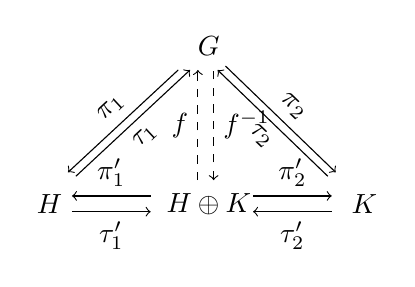
\begin{tikzpicture}
            \node [left] at (0,1) {$H$};
            \node [left] at (2.4,1) {$H\oplus K$};
            \node [left] at (4,1) {$K$};
            \node [left] at (2,3) {$G$};
            \draw [<-] (0,1.1)-- node [above, pos=0.5]{$\pi_{1}'$} (1,1.1);
            \draw [->] (0,0.9)-- node [below, pos=0.5]{$\tau_{1}'$} (1,0.9);
            \draw [->] (2.3,1.1)-- node [above, pos=0.5]{$\pi_{2}'$} (3.3,1.1);
            \draw [<-] (2.3,0.9)-- node [below, pos=0.5]{$\tau_{2}'$} (3.3,0.9);
            \draw [->, dashed] (1.6,1.3)-- node [left, pos=0.5]{$f$} (1.6,2.7);
            \draw [<-, dashed] (1.8,1.3)-- node [right, pos=0.5]{$f^{-1}$} (1.8,2.7);
            \draw [<-] (-0.05,1.4)-- node [above, pos=0.5, sloped]{$\pi_{1}$} (1.35,2.7);
            \draw [->] (0.05,1.35)-- node [below, pos=0.5, sloped]{$\tau_{1}$} (1.5,2.7);
            \draw [<-] (3.35,1.4)-- node [above, pos=0.5, sloped]{$\pi_{2}$} (1.95,2.75);
            \draw [->] (3.25,1.35)-- node [below, pos=0.5, sloped]{$\tau_{2}$} (1.85,2.7);
        \end{tikzpicture}
    \end{figure}
    For $f=\tau_{1}'\pi_{1}+\tau_{2}'\pi_{2}$ which is a well defined homomorphism. $\forall h\in H$ and $k\in K$, $\tau_{1}'(h)+\tau_{2}'(k)=(h,k)\in H\oplus K$. Thus $f(x)=(e_{1},e_{2})$ if and only if $\pi_{1}(x)=e_{1}$ and $\pi_{2}(x)=e_{2}$. $\tau_{1}\pi_{1}(x)+\tau_{2}\pi_{2}(x)=\tau_{1}(e_{1})+\tau_{2}(e_{2})=e=x$. Thus $\mathrm{Ker}f=\{e\}$. $f$ is a monomorphism. $\forall (h,k)\in H\oplus K$, take $x=\tau_{1}(h)+\tau_{2}(k)\in G$, then \[\begin{aligned}
        f(x)&=\tau_{1}'\pi_{1}\tau_{1}(h)+\tau_1'\pi_{1}\tau_{2}(h)+\tau_{2}'\pi_{2}\tau_{1}(k)+\tau_{2}'\pi_{2}\tau_{1}(k)\\&=\tau_{1}'(h)+\tau_{2}'(k)=(h,k)\in H\oplus K
    \end{aligned}\]
    $f$ is a epimorphism. Thus $G\cong H\oplus K$.
\end{answer}

$$ $$

\begin{ex}
    Give an example to show that the weak direct product is not a coproduct in the category of all groups.
\end{ex}

\begin{answer}
    Consider $S_{3}$ and $S_{3}\times S_{3}$.

    \begin{figure}[H]\centering
        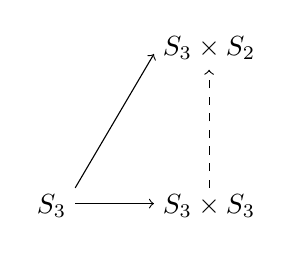
\begin{tikzpicture}
            \node [above] at (0,0) {$S_{3}$};
            \node [above] at (2,0) {$S_{3}\times S_{3}$};
            \node [above] at (2,2) {$S_{3}\times S_{2}$};
            \draw [->] (0.3,0.3) to (1.3,0.3);
            \draw [->] (0.3,0.5) to (1.3,2.2);
            \draw [->, dashed] (2,0.5) to (2,2);
        \end{tikzpicture}
    \end{figure}
    Since there doesn't exist homomorphism $S_{3}\to S_{2}$, there is no homomorphism $S_{3}\times S_{3}\to S_{3}\times S_{2}$.
\end{answer}

$$ $$

\begin{ex}
    Let $G$, $H$ be finite cyclic groups. Then $G\times H$ is cyclic if and only if $(\left| G \right|, \left| H \right|  )=1$.
\end{ex}

\begin{answer}
    Assume $\left| G \right| =m$, $\left| H \right| =n$, then $G\cong Z_{m}$, $H\cong Z_{n}$ and $G\times H\cong Z_{m}\oplus Z_{n}$.
    
    If$(\left| G \right| ,\left| H \right| )=1$. Consider $(x_{1}, x_{2})\in Z_{m}\oplus Z_{n}$. By \emph{Chinese Remainder Theorem}, there exists $x$ such that $a\equiv x\mod \mathrm{lcm}(m,n)$ and $a\equiv x_{1}\mod m$, $a\equiv x_{2}\mod n$. Thus, $a(1,1)=(x_{1},x_{2})$. $Z_{m}\oplus Z_{n}<\left\langle (1,1)\right\rangle$. $\left\langle (1,1)\right\rangle<Z_{m}\oplus Z_{n}$ is trivial. So $Z_{m}\oplus Z_{n}=\left\langle(1,1)\right\rangle\cong G\times H$ is cyclic.

    If $G\times H$ is cyclic. Assume $l=\gcd(m,n)$ and there exist $x$ such that  $x_{1}\equiv x\mod m$, $x_{2}\equiv x\mod n$. Take $x_{1}\not\equiv x_{2}\mod l$, it can be chosen properly. Consider $(x_{1}, x_{2})\in Z_{m}\oplus Z_{n}$, $x=k_{1}m+x_{1}=k_{2}n+x_{2}\Rightarrow x_{1}\equiv x_{2}\mod l$. That's contradictory!
\end{answer}

$$ $$

\begin{ex}
    Every finitely generated abelian group $G\neq\left\langle e\right\rangle$ in which every element (except $e$) has order $p$ ($p$ prime) is isomorphic to $Z_{p}\oplus Z_{p}\oplus\cdots\oplus Z_{p}$($n$ summands) for some $n\geq 1$.
\end{ex}

\begin{answer}
    Assume $\{a_{1}, a_{2}, \dots, a_{n}\}$ generates $G$. $\left| a_{i} \right| =p$ for $i=1,2,\dots, n$  so $\left\langle a_{i}\right\rangle\cong Z_{p}$. Now we show that $G=\prod\limits_{i=1}^{n}{^{w}}\left\langle a_{i}\right\rangle\cong \sum\limits_{i=1}^{n}Z_{p}$. $G=\left\langle a_{1}, a_{2},\dots, a_{n}\right\rangle$ and $\left\langle a_{1}\right\rangle\lhd G$ for $i=1,2,\dots, n$. If exist $\left\langle a_{i}\right\rangle$ s.t. $\prod\limits_{j=1, j\neq i}^{n}\left\langle a_{j}\right\rangle\cap \left\langle a_{i}\right\rangle\neq \{e\}$. Then there exists $a_{i}^{s_{i}}=a_{1}^{s_{1}}\cdots a_{i-1}^{s_{i-1}}a_{i+1}^{s_{i+1}}\cdots a_{n}^{s_{n}}$. $(s_{i},p)=1$ so $\exists 1\leq t_{i}\leq p-1$ such that $s_{i}t_{i}\equiv 1\mod p$. So $a_{i}^{s_{i}t_{i}}=a_{1}^{s_{1}t_{i}}\cdots a_{i-1}^{s_{i-1}t_{i}}a_{i+1}^{s_{i+1}t_{i}}\cdots a_{n}^{s_{n}t_{i}}=a_{i}$. $\{a_{1}, a_{2}, \dots, a_{n}\}$ can generate $G$. That's contradictory! So $\prod\limits_{j=1, j\neq i}^{n}\left\langle a_{j}\right\rangle\cap \left\langle a_{i}\right\rangle=\{e\}$, which means $G=\prod\limits_{i=1}^{n}{^{w}}\left\langle a_{i}\right\rangle\cong \sum\limits_{i=1}^{n}Z_{p}$.
\end{answer}

$$ $$

\begin{ex}
    Let $H,K,N$ be nontrivial normal subgroups of a group $G$ and suppose $G=H\times K$. Prove that $N$ is in the center of $G$ or $N$ intersects one of $H,K$ nontrivially. Give examples to show that both possibilities can actually occur when $G$ is nonabelian.
\end{ex}

\begin{answer}
    If $N\cap H=N\cap K=\{e\}$. $G=HK$. $\forall h\in H$ and $k\in K$, since $H\cap K=\{e\}$, $hk=kh$. For any $hk\in N$, and $h_{1}\in H\subset HK$, $h_{1}^{-1}hkh_{1}=h_{1}^{-1}hh_{1}k\in N$. Assume $h'=h_{1}^{-1}h_{1}\in H$, $h'k\in N$. Thus $h'^{-1}k^{-1}kh=h'^{-1}h\in N$. So $h'^{-1}h=e$, $h=h'$, $h$ is in the center $C(H)$ of group $H$. Similarly, $k\in C(K)$ which is the center of $K$. Then $\forall hk\in N$ and $h_{1}k_{1}\in G$, $k_{1}^{-1}h_{1}^{-1}hkh_{1}k_{1}=h_{1}^{-1}hh_{1}k_{1}^{-1}kk_{1}=hk$. $N\subset N(G)$.

    For $N\cup H\neq \varnothing$, the example can be trivial: $N<H$ and $N\lhd G$. There's many cyclic group satisfy the condition.

    For $N\subset C(G)$. Take $G=D_{4}^{*}\times D_{4}^{*}$, $H=D_{4}^{*}\times \{I\}$, $K=\{I\}\times D_{4}^{*}$. $\{I,R^{2}\}$ is normal in $D_{4}^{*}$. Denote $N$ is the subgroup $\{(I,I), (R^{2},R^{2})\}$. We can verify that $N$ satisfies the condition.
\end{answer}

$$ $$

\begin{ex}
    Corollary 8.7 is false if one of the $N_{i}$ is not normal.
\end{ex}

\begin{answer}
    Consider $N_{1}, N_{2},\dots , N_{n}$ are all finite. WLOG, assume $N_{1}$ is not normal. $G=\left\langle\bigcup\limits_{i=1}^{n}N_{i}\cup N_{1}\right\rangle$ and $N_{1}N_{2}\cdots N_{n}\subset G$. Denote $A=N_{2}N_{3}\cdots N_{n}$. Then $\exists a\in A$ such that $a^{-1}na=n'\notin N_{1}$. Thus $n'a\in G$ but $n'a\notin N_{1}N_{2}\cdots N_{n}$ so $\left| G \right| >\left| N_{1}N_{2}\cdots N_{n} \right| =\left| N_{1} \right|\times\left| N_{2} \right|\times\cdots\times\left| N_{n} \right| =\left| N_{1}\times N_{2}\times\cdots\times N_{n} \right| $.
\end{answer}

$$ $$

\begin{ex}
    If a group $G$ is the (internal) direct product of its subgroups $H$, $K$, then $H\cong G / K$ and $G /H \cong K$.
\end{ex}

\begin{answer}
    $H\cap K=\{e\}$. $G=H\times K=HK$. Thus $HK / H\cong K/(K\cap H)=K$, $HK /K\cong H /(K\cap H)=H$.
\end{answer}

$$ $$

\begin{ex}
    If $\{G_{i}|i\in I\}$ is a family of groups, then $\prod^{w}G_{i}$ is the internal weak product its subgroups $\{\tau_{i}(G_{i})|i\in I\}$.
\end{ex}

\begin{answer}
    Take $\tau_{i}(g)=(e_{1}, e_{2},\dots, g,\dots,e_{n})$, $g\in G_{i}$.$\tau_{i}(G_{i})$. $\tau_{i}(G_{i})$ is normal in $\prod\limits_{i\in I}{^{w}}G_{i}$. $\tau_{i}(G_{i})\cap \tau_{j}(G_{j})=\{(e_{1}, e_{2}, \dots , e_{n})\}$ which is the identity element in $\prod\limits_{i\in I}{^{w}}G_{i}$. $\forall (g_{1}, g_{2},\dots, g_{n})\in \prod\limits_{i\in I}{^{w}}G_{i}$, we have \[(g_{1}, g_{2}, \dots, g_{n})=(g_{1},e_{2},\dots, e_{n})(e_{1}, g_{2}, \dots, e_{n})\cdots(e_{1}, e_{2}, \dots, g_{n})\] Thus $\prod\limits_{i\in I}{^{w}}G_{i}\subset \left\langle\bigcup\limits_{i\in I}{^{w}}\tau_{i}(G_{i})\right\rangle$ and \[\left\langle\bigcup\limits_{i\in I}{^{w}}\tau_{i}(G_{i})\right\rangle=\tau_{1}(G_{1})\tau_{2}(G_{2})\cdots \tau_{n}(G_{n})\subset \prod\limits_{i\in I}{^{w}}G_{i}\] Therefore $\prod\limits_{i\in I}{^{w}}G_{i}$ is the direct product of $\tau_{i}(G_{i})$.
\end{answer}

$$ $$

\begin{ex}
    Let $\{N_{i}|i\in I\}$ be a family of subgroups of a group $G$. Then $G$ is the internal weak product of $\{N_{i}|i\in I\}$if and only if:
    \begin{enumerate}[(i)]
        \item $a_{i}a_{j}=a_{j}a_{i}$ for all $i\neq j$ and $a_{i}\in N_{i}$, $a_{j}\in N_{j}$;
        \item every nonidentity element of $G$ is uniquely a product $a_{i_{1}}\cdots a_{i_{n}}$, where $i_{i},\dots,i_{n}$ are distinct elements of $I$ and $e\neq a_{i_{k}}\in N_{i_{k}}$ for each $k$.
    \end{enumerate}
\end{ex}

\begin{answer}
    Trivial.
\end{answer}

$$ $$

\begin{ex}
    A normal subgroup $H$ of a group $G$ is said to be a \textbf{direct factor} (\textbf{direct summand} if $G$ is additive abelian) if there exists a (normal) subgroup $K$ of $G$ such that $G=H\times K$.
    \begin{enumerate}[(a)]
        \item If $H$ is a direct factor of $K$ and $K$ is a direct factor of $G$, then $H$ is normal in $G$.
        \item If $H$ is a direct factor of $G$, then every homomorphism $H\to G$ may be extended to an endomorphism $G\to G$. However, a monomorphism $H\to G$ need not be extendible to and automorphism $G\to G$.
    \end{enumerate}
\end{ex}

\begin{answer}
    \begin{enumerate}[(a)]
        \item $G=K\times K'= (H\times H')\times K'$. So $\forall g\in G$, $g=hh'k'$ with $h\in H$, $h' \in H'$ and $k'\in K'$. $\forall h_{1}\in H$ and $g\in G$, $g^{-1}h_{1}g=k'^{-1}h'^{-1}h^{-1}h_{1}hh'k'=(h^{-1}h_{1}h)(h'^{-1}h')(k'^{-1}k')=h^{-1}h_{1}h\in H$. Thus $H\lhd G$.
        \item If $G=H\times K$. For a homomorphism $f:H\to G$, we construct a homomorphism $\bar{f}:G\to G$, $\forall g\in G$,$g$ can be uniquely written as $g=hk$ where $h\in H$, $k\in K$. Take $\tau(g)=h$ which is a homomorphism $\tau:G\to H$. We can get $\bar{f}=f\circ\tau: G\to G$ is a endomorphism but it needn't to be a automorphism.
    \end{enumerate}
\end{answer}

$$ $$

\begin{ex}
    Let $\{G_{i}|i\in I\}$ be a family of groups and $J\subset I$. The map $\alpha: \prod\limits_{j\in J}G_{j}\to \prod\limits_{i\in I}G_{i}$ given by $\{a_{j}\}\mapsto \{b_{i}\}$, where $b_{j}=a_{j}$ for $j\in J$ and $b_{i}=e_{i}$(identity in $G_{i}$) for $i\notin J$, is a monomorphism of groups and $\prod\limits_{i\in I}G_{i} /\alpha(\prod\limits_{j\in J}G_{j})\cong \prod\limits_{i\in I-J}G_{i}$.
\end{ex}

\begin{answer}
    Define a map $\beta:\prod\limits_{i\in I}G_{i}\to \prod\limits_{i\in I-J}G_{i}$ given by $\{a_{i}\}\mapsto \{b_{i}\}$ and for those $i\in I-J$, $\exists b_{i}\in \{b_{i}\}$ s.t. $a_{i}=b_{i}$. Thus $\beta(\{a_{i}\})\beta(\{a_{i}'\})=\beta(\{a_{i}a_{i}'\})$, $\beta$ is a well defined homomorphism. $\mathrm{Ker}\beta=\{\{a_{i}\}\in\prod\limits_{i\in I}G_{i}|a_{i}=e_{i} \text{ for }i \in I-J\}=\alpha(\prod\limits_{j\in J}G_{j})$. We verify $\beta$ is a epimorphism. $\forall \{b_{i}\}\in \prod\limits_{i\in I-J}G_{i}$, take $\{a_{i}\}\in \prod\limits_{i\in I}G_{i}$ where $a_{i}=b_{i}$ for $i\in I-J$. Then $\beta(\{a_{i}\})=\{b_{i}\}$. Thus $\beta$ is an isomorphism, $\mathrm{Im}\beta=\prod\limits_{i\in I-J}G_{i}\cong \prod\limits_{i\in I}G_{i} /\alpha(\prod\limits_{j\in J}(G_{j}))$.
\end{answer}

$$ $$

\begin{ex}
    For $i=1,2$ let $H_{i}\lhd G_{i}$ and give examples to show that each of the following statements may be false:
    \begin{enumerate}[(a)]
        \item $G_{1}\cong G_{2}$ and $H_{1}\cong H_{2}\Rightarrow G_{1} /H_{1}\cong G_{2} /H_{2}$.
        \item $G_{1}\cong G_{2}$ and $G_{1}/ H_{1}\cong G_{2} / H_{2}\Rightarrow H_{1}\cong H_{2}$.
        \item $H_{1}\cong H_{2}$ and $G_{1}/ H_{1}\cong G_{2} / H_{2}\Rightarrow G_{1}\cong G_{2}$.
    \end{enumerate}
\end{ex}

\begin{answer}
    \begin{enumerate}[(a)]
        \item Take $G_{1}=G_{2}=Z_{2}\times Z_{4}$, $H_{1}=Z_{2}\times \{\bar{0}\}$, $H_{2}=\{(\bar{0},\bar{0}), (\bar{0}, \bar{2})\}$.
        \item Take $G_{1}=G_{2}=Z_{2}\times Z_{4}$, $H_{1}=\{\bar{0}\}\times Z_{4}$, $H_{2}=\{(\bar{0}, \bar{0}), (\bar{1}, \bar{0}), (\bar{0}, \bar{2}), \\(\bar{1}, \bar{2})\}$.
        \item Take $H_{1}=\{(\bar{0},\bar{0}), (\bar{0},\bar{2})\}$, $H_{2}=Z_{2}$ and $G_{1}=Z_{2}\times Z_{4}$, $G_{2}=Z_{2}\times K_{4}$.
    \end{enumerate}
\end{answer}